\documentclass{standalone}
\usepackage{tikz}

\newcommand{\bt}{\mathbf{t}}
\newcommand{\bx}{\mathbf{x}}
\newcommand{\by}{\mathbf{y}}
\newcommand{\bz}{\mathbf{z}}
\newcommand{\eq}{=}




\begin{document}
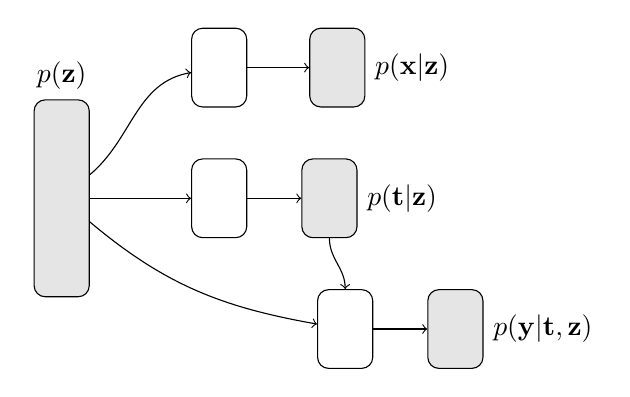
\begin{tikzpicture}
    \node[draw, minimum width=0.7cm, minimum height=2.5cm, rounded corners, label=$p(\bz)$, fill=black!10!white] (z) at (0, 0) {};
    \node[draw, minimum width=0.7cm, minimum height=1cm, rounded corners] (z1) at (2, 1.66) {};
    \node[draw, minimum width=0.7cm, minimum height=1cm, rounded corners] (z2) at (2, 0) {};
    \node[draw, minimum width=0.7cm, minimum height=1cm, rounded corners] (z3) at (3.6, -1.66) {};
    % \node[draw, minimum width=0.7cm, minimum height=1cm, rounded corners] (z4) at (2, -2) {};
    
    \node[draw, minimum width=0.7cm, minimum height=1cm, rounded corners, label=right:$p(\bx|\bz)$,fill=black!10!white] (x) at (3.5, 1.66) {};
    % \node[draw, circle, inner sep=0.08cm] (switch1) at (4, 0.66) {};
    \node[draw, minimum width=0.7cm, minimum height=1cm, rounded corners, label=right:$p(\bt|\bz)$,fill=black!10!white] (t) at (3.4, -0.0) {};
    % \node[draw, circle, inner sep=0.08cm] (switch2) at (4, -2) {};
    
    
    % \node[draw, minimum width=0.7cm, minimum height=1cm, rounded corners] (z21) at (6, 0.66) {};
    % \node[draw, minimum width=0.7cm, minimum height=1cm, rounded corners] (z31) at (6, -2) {};
    
    \node[draw, minimum width=0.7cm, minimum height=1cm, rounded corners, label=right:{$p(\by|\bt, \bz)$},fill=black!10!white] (yt) at (5, -1.66) {};
    % \node[draw, minimum width=0.7cm, minimum height=1cm, rounded corners, , label=right:{$p(\by|\bt \eq 1, \bz)$},fill=black!10!white] (yt1) at (8, -2) {};
    
    \draw[->, out=40, in=190] (z) to (z1);
    \draw[->] (z) to (z2);
    \draw[->, out=-40, in=170] (z) to (z3);
    % \draw[->] (z) to (z4);

    \draw[->] (z1) to (x);
    % \draw[->] (z2) to (switch1);
    \draw[->] (z2) to (t);
    % \draw[->] (z4) to (switch2);
    \draw[->, out=-90, in=90] (t) to (z3);
    % \draw[->] (t) to (switch1);
    
    % \draw[->] (switch1) to (z21);
    % \draw[->] (switch2) to (z31);
    % \draw[->] (z21) to (yt0);
    \draw[->] (z3) to (yt);
    
\end{tikzpicture}
\end{document}